%!TEX root = ../main.tex

\todo Write up something about the experimental setup

\section{Calibration of a multichannel analyser}
\label{sec:ecal}

\begin{figure}
	\label{fig:ecal-plot}
	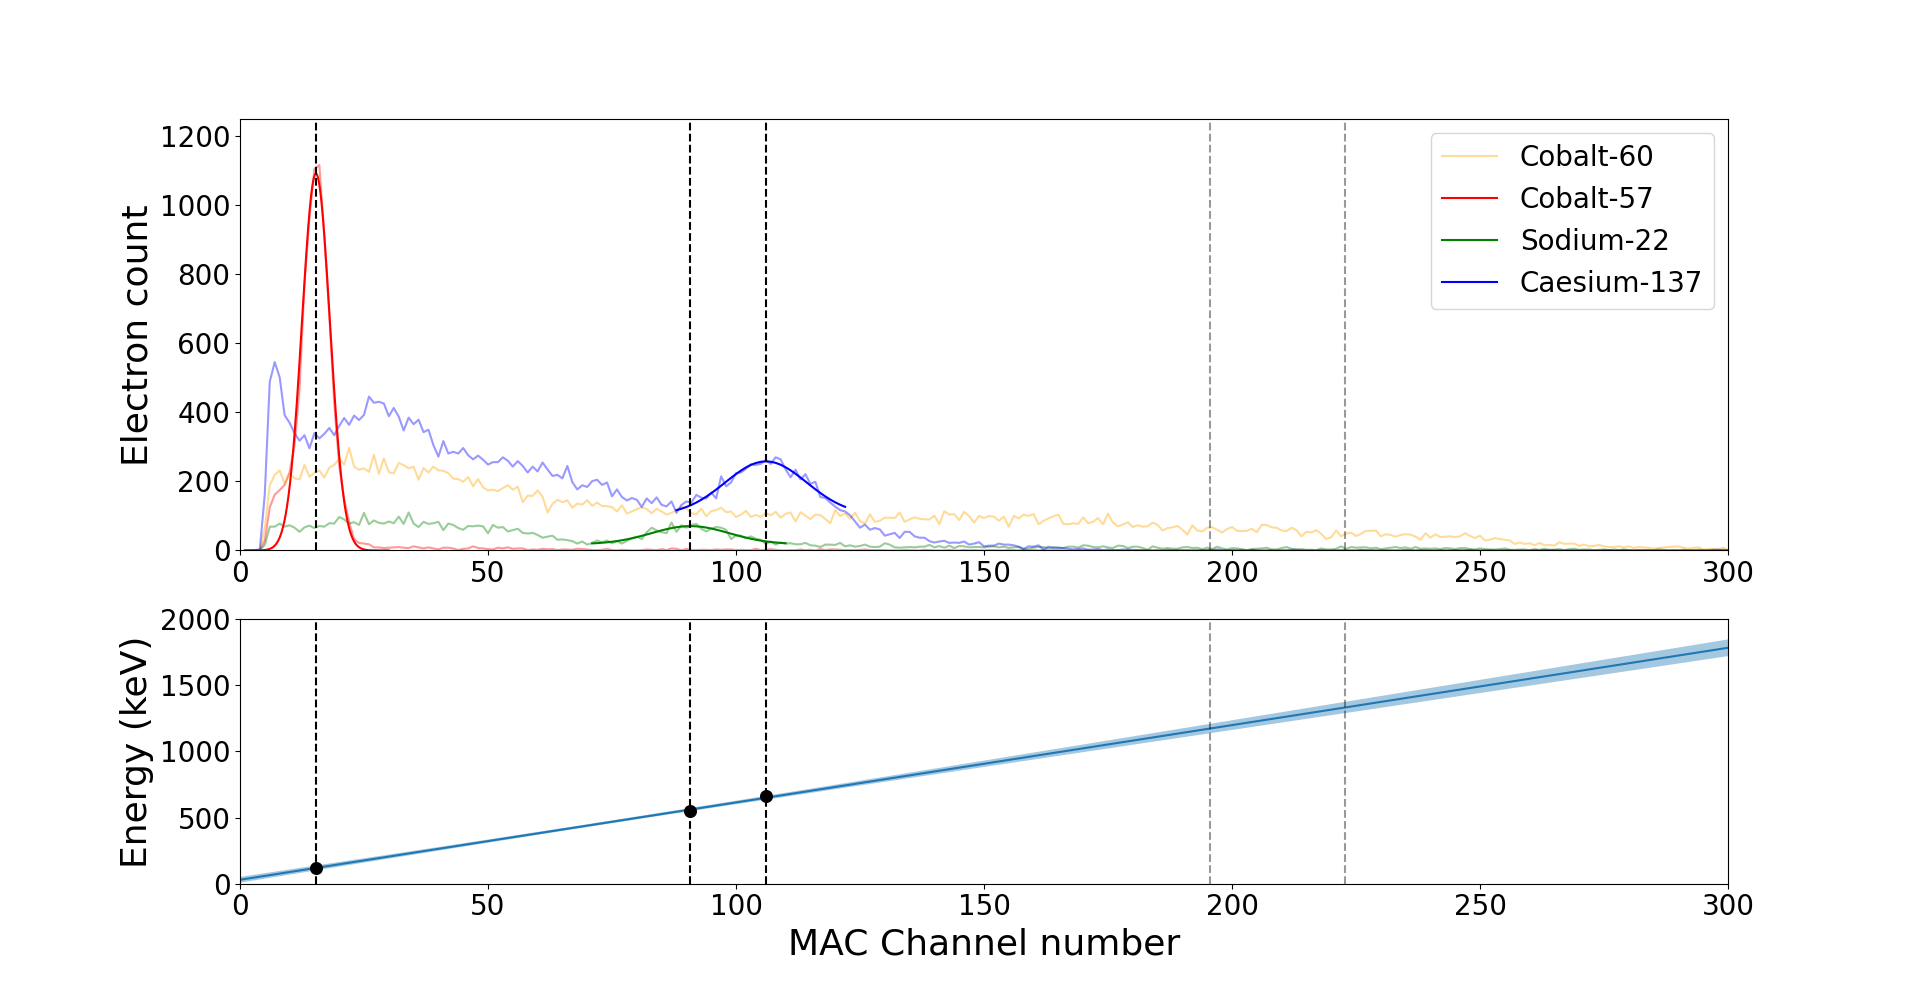
\includegraphics[width=1.0\textwidth]{./fig/ecal-plot.png}
	\caption{}{The gamma spectra of various radionuclides as measured by the MAC
	is depicted in the upper plot. A Gaussian fit hightlights the characteristic
	photopeaks for each (except Co-60, see text) measurement. The lower plot
	sets the measured channel numbers into context with the energies of the
	observed transitions. A linear model that connects MAC channel number with an
	energy is established.}
\end{figure}

As a first task the MAC needs to be calibrated so that measured channel numbers of an
event can be related to the energy of the particles that caused it. The presented
calibration is fourfold. In seperate measurements the radionuclides Cobalt-57, and
-60, as well as Sodium-22, and Caesium-137 are placed in front of the
NaJ-scintillator. Their $\gamma$-spectrum is measured for \SI{300}{\second}. The
resulting distribution of observed events across the different measuring channels is
depicted in \autoref{fig:ecal-plot}. The interesting parts of the spectra are the
gaussian shaped sections located at the tail ends. They represent the photopeaks
discussed briefly in \autoref{sec:compton-spectrum}.

Equipped with theoretical knowledge of the radioactive processes, one can compare the
measured channel with the expected energy of a nuclear transition to establish a
linear connection between the two. For more solid statistics this calibration is done
simultanously for all measured radionuclides. Below listed in
\autoref{tab:transitions} are the different observed radioactive transitions, the
channel they were measured in by the MAC, as well as the corresponding energy of the
transition. In the bottom plot of \autoref{fig:ecal-plot} these results are
visualised.
